% document formatting
\documentclass[10pt]{article}
\usepackage[utf8]{inputenc}
\usepackage[left=1in,right=1in,top=1in,bottom=1in]{geometry}
\usepackage[T1]{fontenc}
\usepackage{xcolor}

% math symbols, etc.
\usepackage{amsmath, amsfonts, amssymb, amsthm}

% lists
\usepackage{enumerate}

% images
\usepackage{graphicx} % for images
\usepackage{tikz}

% code blocks
% \usepackage{minted, listings} 

% verbatim greek
\usepackage{alphabeta}

\graphicspath{{./assets/images/Week 2}}

\title{02-613 Week 2 \\ \large{Algorithms and Advanced Data Structures}}
 
\author{Aidan Jan}

\date{\today}

\begin{document}
\maketitle

\section*{Union-Find Abstract Data Type}
In Kruskal's algorithm, we need a data structure to quickly find cycles.  We need a way to:
\begin{itemize}
    \item quickly determine which subgraph a given node is in
    \item quickly merge two subgraphs
    \item a constructor for the data structure
\end{itemize}
One data structure we can use is the Union-Find data structure.  What we basically do is store a collection of trees.
\begin{itemize}
    \item Create a struct for a node, containing the connections for the graph in an array, but also, each has an additional variable, a parent pointer.
    \item To determine which group the node is in, follow the parent pointers up until you get to a node with no parent pointer.  (This gives every subgraph a unique identifier.)
    \item To merge two groups, simply take the root of the smaller tree, and add the root of the bigger tree as a parent to the smaller tree.
    \begin{itemize}
        \item To do this quickly, we need a size array.  Without size array would be O($n$).  With size array would be O($1$).
    \end{itemize}
\end{itemize}
\begin{tikzpicture}[
    level distance=1.5cm,
    level 1/.style={sibling distance=2cm},
    level 2/.style={sibling distance=1cm},
    every node/.style={circle, draw, minimum size=8mm, inner sep=0pt}
]
\node (placeholder) [opacity=0] at (-4, 0) {};

\begin{scope}[shift={(0,0)}]
\node {1}
    child {
        node {3}
        child {node {10}}
    }
    child {
        node {4}
    };
\end{scope}

\begin{scope}[shift={(4,0)}] 
\node {2}
    child {node {9}}
    child {node {6}};
\end{scope}

\begin{scope}[shift={(7,0)}] 
    \node {5};
\end{scope}

\begin{scope}[shift={(9,0)}] 
    \node {7}
        child {node {8}};
    \end{scope}

\draw[dashed] (3.6, 0) -- (0.4, 0);

\end{tikzpicture}
\begin{itemize}
    \item In the diagram above, to find the node's group, simply follow the tree up to the root.  The root is the node's group.
    \item In the image above, we would merge trees 1 and 2 by making the parent of node 2 node 1.  (see dotted line)
\end{itemize}
We can actually optimize this further if we convert the structs to arrays.  The below image represents the same structure as above:
\pagebreak

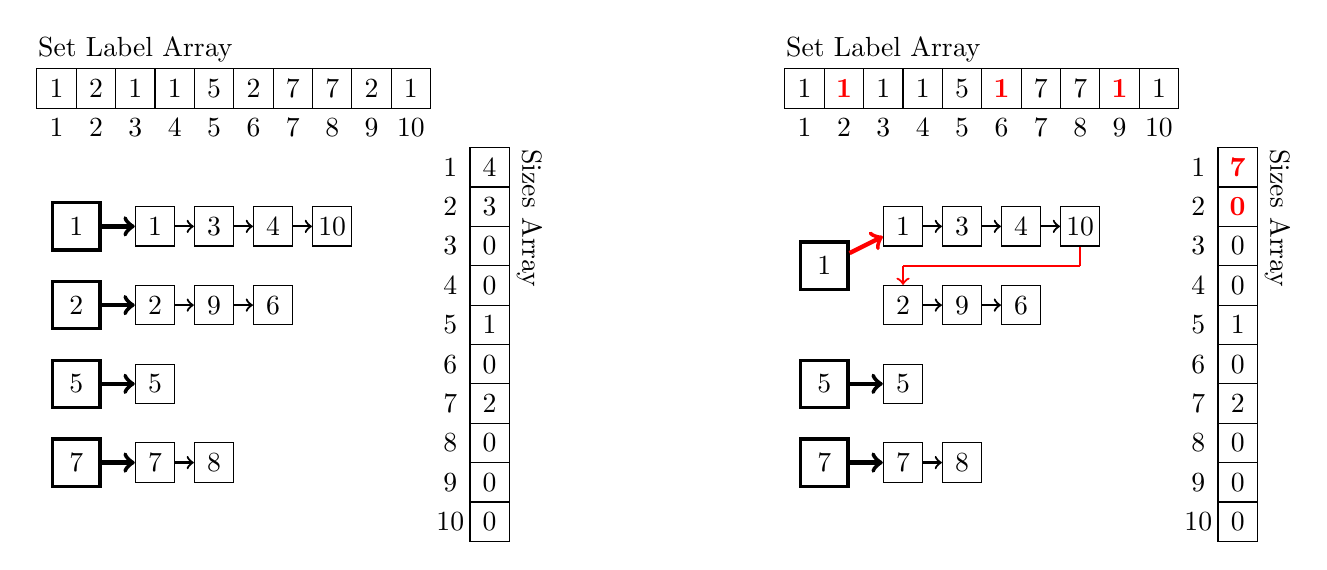
\begin{tikzpicture}
    \node (0, 0) (origin) {};
    % set label array
    \node[align=left] at (1.25, 0.75) (setLabelArray) {Set Label Array};
    \foreach \i in {1,...,10} {
        \node[align=left] at ({-0.25 + 0.5 * \i}, -0.25) (label\i) {\the\numexpr\i\relax};
    }
    \draw (0, 0) rectangle (5, 0.5);
    \foreach \i in {0,...,8} {
        \draw ({0.5 + 0.5 * \i}, 0) -- ({0.5 + 0.5 * \i}, 0.5);
    }
    \foreach [count=\i] \val in {1,2,1,1,5,2,7,7,2,1} {
        \node at ({0.25 + 0.5*(\i-1)}, 0.25) (lind\i) {\val};
    }

    % sizes array
    \node[align=left, rotate=270] at (6.25, -1.4) (sizesArray) {Sizes Array};
    \foreach \i in {1,...,10} {
        \node[align=left] at (5.25, {-0.25 - 0.5 * \i}) (size\i) {\the\numexpr\i\relax};
    }
    \draw (5.5, -0.5) rectangle (6, -5.5);
    \foreach \i in {0,...,8} {
        \draw (5.5, {-1 - 0.5 * \i}) -- (6, {-1 - 0.5 * \i});
    }
    \node at (5.75, -0.75) (sind1) {4};
    \node at (5.75, -1.25) (sind2) {3};
    \node at (5.75, -1.75) (sind3) {0};
    \node at (5.75, -2.25) (sind4) {0};
    \node at (5.75, -2.75) (sind5) {1};
    \node at (5.75, -3.25) (sind6) {0};
    \node at (5.75, -3.75) (sind7) {2};
    \node at (5.75, -4.25) (sind8) {0};
    \node at (5.75, -4.75) (sind9) {0};
    \node at (5.75, -5.25) (sind10) {0};

    % items labels
    \node[draw, rectangle, very thick, minimum width=0.6cm, minimum height=0.6cm] at (0.5, -1.5) (objecth1) {1};
    \node[draw, rectangle, very thick, minimum width=0.6cm, minimum height=0.6cm] at (0.5, -2.5) (objecth2) {2};
    \node[draw, rectangle, very thick, minimum width=0.6cm, minimum height=0.6cm] at (0.5, -3.5) (objecth5) {5};
    \node[draw, rectangle, very thick, minimum width=0.6cm, minimum height=0.6cm] at (0.5, -4.5) (objecth7) {7};

    % items
    \node[draw, rectangle, minimum width=0.5cm, minimum height=0.5cm, inner sep=0mm] at (1.5, -1.5) (object1) {1};
    \node[draw, rectangle, minimum width=0.5cm, minimum height=0.5cm, inner sep=0mm] at (2.25, -1.5) (object3) {3};
    \node[draw, rectangle, minimum width=0.5cm, minimum height=0.5cm, inner sep=0mm] at (3, -1.5) (object4) {4};
    \node[draw, rectangle, minimum width=0.5cm, minimum height=0.5cm, inner sep=0mm] at (3.75, -1.5) (object10) {10};
    \node[draw, rectangle, minimum width=0.5cm, minimum height=0.5cm, inner sep=0mm] at (1.5, -2.5) (object2) {2};
    \node[draw, rectangle, minimum width=0.5cm, minimum height=0.5cm, inner sep=0mm] at (2.25, -2.5) (object9) {9};
    \node[draw, rectangle, minimum width=0.5cm, minimum height=0.5cm, inner sep=0mm] at (3, -2.5) (object6) {6};
    \node[draw, rectangle, minimum width=0.5cm, minimum height=0.5cm, inner sep=0mm] at (1.5, -3.5) (object5) {5};
    \node[draw, rectangle, minimum width=0.5cm, minimum height=0.5cm, inner sep=0mm] at (1.5, -4.5) (object7) {7};
    \node[draw, rectangle, minimum width=0.5cm, minimum height=0.5cm, inner sep=0mm] at (2.25, -4.5) (object8) {8};

    \draw[ultra thick, ->] (objecth1) edge (object1);
    \draw[thick, ->] (object1) edge (object3);
    \draw[thick, ->] (object3) edge (object4);
    \draw[thick, ->] (object4) edge (object10);

    \draw[ultra thick, ->] (objecth2) edge (object2);
    \draw[thick, ->] (object2) edge (object9);
    \draw[thick, ->] (object9) edge (object6);

    \draw[ultra thick, ->] (objecth5) edge (object5);
    \draw[ultra thick, ->] (objecth7) edge (object7);
    \draw[thick, ->] (object7) edge (object8);

    % set label array 2
    \node[align=left] at (10.75, 0.75) (setLabelArray_) {Set Label Array};
    \node[align=left] at (9.75, -0.25) (label0_) {1};
    \node[align=left] at (10.25, -0.25) (label1_) {2};
    \node[align=left] at (10.75, -0.25) (label2_) {3};
    \node[align=left] at (11.25, -0.25) (label3_) {4};
    \node[align=left] at (11.75, -0.25) (label4_) {5};
    \node[align=left] at (12.25, -0.25) (label5_) {6};
    \node[align=left] at (12.75, -0.25) (label6_) {7};
    \node[align=left] at (13.25, -0.25) (label7_) {8};
    \node[align=left] at (13.75, -0.25) (label8_) {9};
    \node[align=left] at (14.25, -0.25) (label9_) {10};
    \draw (9.5, 0) rectangle (14.5, 0.5);
    \draw (10, 0) -- (10, 0.5);
    \draw (10.5, 0) -- (10.5, 0.5);
    \draw (11, 0) -- (11, 0.5);
    \draw (11.5, 0) -- (11.5, 0.5);
    \draw (12, 0) -- (12, 0.5);
    \draw (12.5, 0) -- (12.5, 0.5);
    \draw (13, 0) -- (13, 0.5);
    \draw (13.5, 0) -- (13.5, 0.5);
    \draw (14, 0) -- (14, 0.5);
    \node at (9.75, 0.25) (lind1_) {1};
    \node at (10.25, 0.25) (lind2_) {\textbf{\textcolor{red}{1}}};
    \node at (10.75, 0.25) (lind3_) {1};
    \node at (11.25, 0.25) (lind4_) {1};
    \node at (11.75, 0.25) (lind5_) {5};
    \node at (12.25, 0.25) (lind6_) {\textbf{\textcolor{red}{1}}};
    \node at (12.75, 0.25) (lind7_) {7};
    \node at (13.25, 0.25) (lind8_) {7};
    \node at (13.75, 0.25) (lind9_) {\textbf{\textcolor{red}{1}}};
    \node at (14.25, 0.25) (lind10_) {1};

    % sizes array 2
    \node[align=left, rotate=270] at (15.75, -1.4) (sizesArray_) {Sizes Array};
    \node[align=left] at (14.75, -0.75) (size1_) {1};
    \node[align=left] at (14.75, -1.25) (size2_) {2};
    \node[align=left] at (14.75, -1.75) (size3_) {3};
    \node[align=left] at (14.75, -2.25) (size4_) {4};
    \node[align=left] at (14.75, -2.75) (size5_) {5};
    \node[align=left] at (14.75, -3.25) (size6_) {6};
    \node[align=left] at (14.75, -3.75) (size7_) {7};
    \node[align=left] at (14.75, -4.25) (size8_) {8};
    \node[align=left] at (14.75, -4.75) (size9_) {9};
    \node[align=left] at (14.75, -5.25) (size10_) {10};
    \draw (15, -0.5) rectangle (15.5, -5.5);
    \draw (15, -1) -- (15.5, -1);
    \draw (15, -1.5) -- (15.5, -1.5);
    \draw (15, -2) -- (15.5, -2);
    \draw (15, -2.5) -- (15.5, -2.5);
    \draw (15, -3) -- (15.5, -3);
    \draw (15, -3.5) -- (15.5, -3.5);
    \draw (15, -4) -- (15.5, -4);
    \draw (15, -4.5) -- (15.5, -4.5);
    \draw (15, -5) -- (15.5, -5);
    \node at (15.25, -0.75) (sind1_) {\textbf{\textcolor{red}{7}}};
    \node at (15.25, -1.25) (sind2_) {\textbf{\textcolor{red}{0}}};
    \node at (15.25, -1.75) (sind3_) {0};
    \node at (15.25, -2.25) (sind4_) {0};
    \node at (15.25, -2.75) (sind5_) {1};
    \node at (15.25, -3.25) (sind6_) {0};
    \node at (15.25, -3.75) (sind7_) {2};
    \node at (15.25, -4.25) (sind8_) {0};
    \node at (15.25, -4.75) (sind9_) {0};
    \node at (15.25, -5.25) (sind10_) {0};

    % items labels 2
    \node[draw, rectangle, very thick, minimum width=0.6cm, minimum height=0.6cm] at (10, -2) (objecth1_) {1};
    \node[draw, rectangle, very thick, minimum width=0.6cm, minimum height=0.6cm] at (10, -3.5) (objecth5_) {5};
    \node[draw, rectangle, very thick, minimum width=0.6cm, minimum height=0.6cm] at (10, -4.5) (objecth7_) {7};

    % items 2
    \node[draw, rectangle, minimum width=0.5cm, minimum height=0.5cm, inner sep=0mm] at (11, -1.5) (object1_) {1};
    \node[draw, rectangle, minimum width=0.5cm, minimum height=0.5cm, inner sep=0mm] at (11.75, -1.5) (object3_) {3};
    \node[draw, rectangle, minimum width=0.5cm, minimum height=0.5cm, inner sep=0mm] at (12.5, -1.5) (object4_) {4};
    \node[draw, rectangle, minimum width=0.5cm, minimum height=0.5cm, inner sep=0mm] at (13.25, -1.5) (object10_) {10};
    \node[draw, rectangle, minimum width=0.5cm, minimum height=0.5cm, inner sep=0mm] at (11, -2.5) (object2_) {2};
    \node[draw, rectangle, minimum width=0.5cm, minimum height=0.5cm, inner sep=0mm] at (11.75, -2.5) (object9_) {9};
    \node[draw, rectangle, minimum width=0.5cm, minimum height=0.5cm, inner sep=0mm] at (12.5, -2.5) (object6_) {6};
    \node[draw, rectangle, minimum width=0.5cm, minimum height=0.5cm, inner sep=0mm] at (11, -3.5) (object5_) {5};
    \node[draw, rectangle, minimum width=0.5cm, minimum height=0.5cm, inner sep=0mm] at (11, -4.5) (object7_) {7};
    \node[draw, rectangle, minimum width=0.5cm, minimum height=0.5cm, inner sep=0mm] at (11.75, -4.5) (object8_) {8};

    \draw[ultra thick, ->, red] (objecth1_) edge (object1_);
    \draw[thick, ->] (object1_) edge (object3_);
    \draw[thick, ->] (object3_) edge (object4_);
    \draw[thick, ->] (object4_) edge (object10_);

    \draw[thick, red] (object10_) edge (13.25, -2);
    \draw[thick, red] (13.25, -2) edge (11, -2);
    \draw[thick, <-, red] (object2_) edge (11, -2);
    \draw[thick, ->] (object2_) edge (object9_);
    \draw[thick, ->] (object9_) edge (object6_);

    \draw[ultra thick, ->] (objecth5_) edge (object5_);
    \draw[ultra thick, ->] (objecth7_) edge (object7_);
    \draw[thick, ->] (object7_) edge (object8_);
\end{tikzpicture} 
\begin{itemize}
    \item The diagram on the right shows the result after merging groups 1 and 2.  Since 2 is a smaller group, it is merged into 1.  Notice the changes in the set label and sizes array.
    \item This increases the speed of the find operation from O($\log n$) to O($1$).
    \item However, this decreases the speed of the union operation from O($1$) to O($k \log k$), where $k$ is the number of unions that has occurred before.
    \item This is an upgrade since we will likely use the find operation much more than the union operation.
\end{itemize}
\subsubsection*{Aside: theorem}
After $k$ unions on $n$ items, O($k \log k$) total time.\\
\begin{proof}
    $k$ unions touches at most $2k$ items, and any item $v$ is relabeled $\log_2(2k)$ times.  This is because we start with each vertex in its own group, and every union at maximum doubles its size.  As a result, each union has $2k \log_2(2k)$ of work, which is O($k \log k$).  In the worst case, this converges to O($\log n$).
\end{proof}
\subsection*{Kruskal's Runtime}
With this data structure, we can now calculate the running time of Kruskal's algorithm:
\begin{itemize}
    \item Sort the edges: O($m \log m$)
    \item Test every edge: O($m$) edges $\times$ (2 $\cdot$ \texttt{find()}) + \texttt{union()}
    \item Therefore, the total time is O($m \log m + 2m + m \log n$).  Since there are more edges than vertices, the O($m \log m$) dominates.  Sorting the edges takes the longest amount of time.
\end{itemize}

\section*{Heaps}
A \textbf{heap} is a data structure that has the ability to provide the smallest (or largest) value in constant time.  For example, a series of integers can be added to the heap, one at a time, and removing the root of the heap would provide the values back in increasing order.  One inspiration of this structure requires us to go back to Prim's Algorithm.

\subsection*{Implementation of Prim's Algorithm}
\begin{enumerate}
	\item Define \texttt{distToT[]} as an array of length \texttt{numVertices}, and initialize every value to \texttt{INTEGER\_MAX}
	\item Let \texttt{u} be an arbitrary node
	\item Set \texttt{distToT[u] = INTEGER\_MIN}
	\item Set \texttt{distToT[v] = d(u, v)} if smaller for $v \in \text{Neighbors}(v)$
	\item Set \texttt{parent(v) = v} if updated
	\item Set \texttt{u = ClosestVertex(T)}
	\item While \texttt{v} exists, go to (3).
\end{enumerate}

\subsubsection*{Aside: Asymptotics}
Asymptotics is a way of measuring running time relative to input size.  This is often written as the Big-O notation.
\begin{itemize}
	\item $x = 4 \cdot y$ is O(1), since no matter the inputs, there are 2 operations.  ($\cdot$ and $=$).  The exact number of operations does not matter, just that it is a constant.
	\item $\forall i \::\: z[i] = 4 + w[i]$ is O(n), since there are 2 times $|z|$ operations.  The number of operations scales with the length of $|z|$, or $n$.
	\item $\forall i, j \::\: a[i] = b[i] \cdot b[j]$ is O($n^2$), since there are $2 \cdot |b| \cdot |b|$ operations.
\end{itemize}
Remember that what we care about is not the exact number of operations, but rather what the operation count curve would look like as the number of elements approaches infinity.  Therefore, a line with $2n$ operations and one with $3n$ operations are both O($n$), since when approaching infinity, they are both straight lines.  Similarly, a function with $n^2$ operations and $n^2 + 500n$ operations are also both O($n^2$), since when approaching infinity, the $n^2$ term will dwarf the $500n$ term, so they are both O($n^2$).
\begin{itemize}
	\item You can always drop the coefficient and terms that are not of the highest power when writing Big-O notation.
	\item Some other consequences of this include that 
	\begin{itemize}
	    \item Factorial time is worse than Exponential time, which is worse than any polynomial time.  In polynomial time, higher powers are worse than lower powers.  
        \item $\log(n)$ lies between constant time and $n$, so by the same logic, $\log(n)$ is better than $n$, and $n\log(n)$ is better than $n^2$
        \item Since coefficients can be dropped, O($\log_2(n)$) and O($\log_3(n)$) are actually equivalent.
    \end{itemize}
\end{itemize}
\rule{\textwidth}{0.4pt}
Going back to Prim's algorithm, if we do the runtime analysis, the slowest steps are steps 4-6, which without including the loop, takes O($m$).  With the loop, it is O($m \cdot n$).  Can we improve this?
\begin{itemize}
	\item The issue is that when we search for the closest vertex using an array, we have to search every vertex of the graph, which is why that specific step is O($m$).  
	\item We can make this faster!  This goes back to the heap.
\end{itemize}
As it turns out, the heap allows you to get the smallest value in the entire array in O($1$) time.  This is much faster than O($n$).

\subsection*{Heap Structure}
A heap uses a binary tree structure, where the smallest element is always at the root.  Suppose we want the smallest element.  This is O($1$) time since we can just extract the root!  However, we have to do some other things to maintain the structure.
\begin{itemize}
	\item Find() is O($1$), as described.
	\item Insert() is O($\log n$).
	\begin{itemize}
	    \item First, insert node as a leaf at the bottom of the tree.
	    \item If that node is smaller than its parent, swap its position with its parent.
	    \item Repeat until the node's value is larger than its parent.
	    \item Note that to optimize the number of times to "bubble" up, we need an array to keep track of pointers to the leaves for quick access, but also to ensure the lengths of all the branches are approximately equal.
    \end{itemize}
    \item Delete() is also O($\log n$)
    \begin{itemize}
        \item Pop the node to be deleted (often the root).
        \item Replace the node with the \textit{smaller} child, if there is one.
        \item Repeat until there are no more children.
    \end{itemize}
\end{itemize}
Delete and insert are O($\log n$) since they are dependent on the depth of the tree.  Since the tree is (ideally) a complete, binary tree, the height is on the order of $\log n$, where $n$ is the number of nodes in the tree.
[insert diagrams for delete/insert]

Note that a heap can be stored in an array.
\end{document}